\documentclass[twoside]{book}

% Packages required by doxygen
\usepackage{calc}
\usepackage{doxygen}
\usepackage{graphicx}
\usepackage[utf8]{inputenc}
\usepackage{makeidx}
\usepackage{multicol}
\usepackage{multirow}
\usepackage{textcomp}
\usepackage[table]{xcolor}

% Font selection
\usepackage[T1]{fontenc}
\usepackage{mathptmx}
\usepackage[scaled=.90]{helvet}
\usepackage{courier}
\usepackage{amssymb}
\usepackage{sectsty}
\renewcommand{\familydefault}{\sfdefault}
\allsectionsfont{%
  \fontseries{bc}\selectfont%
  \color{darkgray}%
}
\renewcommand{\DoxyLabelFont}{%
  \fontseries{bc}\selectfont%
  \color{darkgray}%
}

% Page & text layout
\usepackage{geometry}
\geometry{%
  a4paper,%
  top=2.5cm,%
  bottom=2.5cm,%
  left=2.5cm,%
  right=2.5cm%
}
\tolerance=750
\hfuzz=15pt
\hbadness=750
\setlength{\emergencystretch}{15pt}
\setlength{\parindent}{0cm}
\setlength{\parskip}{0.2cm}
\makeatletter
\renewcommand{\paragraph}{%
  \@startsection{paragraph}{4}{0ex}{-1.0ex}{1.0ex}{%
    \normalfont\normalsize\bfseries\SS@parafont%
  }%
}
\renewcommand{\subparagraph}{%
  \@startsection{subparagraph}{5}{0ex}{-1.0ex}{1.0ex}{%
    \normalfont\normalsize\bfseries\SS@subparafont%
  }%
}
\makeatother

% Headers & footers
\usepackage{fancyhdr}
\pagestyle{fancyplain}
\fancyhead[LE]{\fancyplain{}{\bfseries\thepage}}
\fancyhead[CE]{\fancyplain{}{}}
\fancyhead[RE]{\fancyplain{}{\bfseries\leftmark}}
\fancyhead[LO]{\fancyplain{}{\bfseries\rightmark}}
\fancyhead[CO]{\fancyplain{}{}}
\fancyhead[RO]{\fancyplain{}{\bfseries\thepage}}
\fancyfoot[LE]{\fancyplain{}{}}
\fancyfoot[CE]{\fancyplain{}{}}
\fancyfoot[RE]{\fancyplain{}{\bfseries\scriptsize Generated on Mon Oct 14 2013 19\-:59\-:23 for S\-E\-P2 by Doxygen }}
\fancyfoot[LO]{\fancyplain{}{\bfseries\scriptsize Generated on Mon Oct 14 2013 19\-:59\-:23 for S\-E\-P2 by Doxygen }}
\fancyfoot[CO]{\fancyplain{}{}}
\fancyfoot[RO]{\fancyplain{}{}}
\renewcommand{\footrulewidth}{0.4pt}
\renewcommand{\chaptermark}[1]{%
  \markboth{#1}{}%
}
\renewcommand{\sectionmark}[1]{%
  \markright{\thesection\ #1}%
}

% Indices & bibliography
\usepackage{natbib}
\usepackage[titles]{tocloft}
\setcounter{tocdepth}{3}
\setcounter{secnumdepth}{5}
\makeindex

% Hyperlinks (required, but should be loaded last)
\usepackage{ifpdf}
\ifpdf
  \usepackage[pdftex,pagebackref=true]{hyperref}
\else
  \usepackage[ps2pdf,pagebackref=true]{hyperref}
\fi
\hypersetup{%
  colorlinks=true,%
  linkcolor=blue,%
  citecolor=blue,%
  unicode%
}

% Custom commands
\newcommand{\clearemptydoublepage}{%
  \newpage{\pagestyle{empty}\cleardoublepage}%
}


%===== C O N T E N T S =====

\begin{document}

% Titlepage & ToC
\hypersetup{pageanchor=false}
\pagenumbering{roman}
\begin{titlepage}
\vspace*{7cm}
\begin{center}%
{\Large S\-E\-P2 }\\
\vspace*{1cm}
{\large Generated by Doxygen 1.8.5}\\
\vspace*{0.5cm}
{\small Mon Oct 14 2013 19:59:23}\\
\end{center}
\end{titlepage}
\clearemptydoublepage
\tableofcontents
\clearemptydoublepage
\pagenumbering{arabic}
\hypersetup{pageanchor=true}

%--- Begin generated contents ---
\chapter{S\-E2\-P}
\label{md__r_e_a_d_m_e}
\hypertarget{md__r_e_a_d_m_e}{}
\input{md__r_e_a_d_m_e}
\chapter{Namespace Index}
\section{Namespace List}
Here is a list of all namespaces with brief descriptions\-:\begin{DoxyCompactList}
\item\contentsline{section}{\hyperlink{namespacethread}{thread} }{\pageref{namespacethread}}{}
\end{DoxyCompactList}

\chapter{Hierarchical Index}
\section{Class Hierarchy}
This inheritance list is sorted roughly, but not completely, alphabetically\-:\begin{DoxyCompactList}
\item \contentsline{section}{H\-A\-L}{\pageref{class_h_a_l}}{}
\item \contentsline{section}{thread\-:\-:H\-A\-W\-Thread}{\pageref{classthread_1_1_h_a_w_thread}}{}
\begin{DoxyCompactList}
\item \contentsline{section}{thread\-:\-:Thread}{\pageref{classthread_1_1_thread}}{}
\end{DoxyCompactList}
\item \contentsline{section}{Mutex}{\pageref{class_mutex}}{}
\end{DoxyCompactList}

\chapter{Class Index}
\section{Class List}
Here are the classes, structs, unions and interfaces with brief descriptions\-:\begin{DoxyCompactList}
\item\contentsline{section}{\hyperlink{class_h_a_l}{H\-A\-L} }{\pageref{class_h_a_l}}{}
\item\contentsline{section}{\hyperlink{classthread_1_1_h_a_w_thread}{thread\-::\-H\-A\-W\-Thread} }{\pageref{classthread_1_1_h_a_w_thread}}{}
\item\contentsline{section}{\hyperlink{class_mutex}{Mutex} }{\pageref{class_mutex}}{}
\item\contentsline{section}{\hyperlink{classthread_1_1_thread}{thread\-::\-Thread} }{\pageref{classthread_1_1_thread}}{}
\end{DoxyCompactList}

\chapter{File Index}
\section{File List}
Here is a list of all files with brief descriptions\-:\begin{DoxyCompactList}
\item\contentsline{section}{Software/\-S\-E2\-P2/\hyperlink{main_8cc}{main.\-cc} }{\pageref{main_8cc}}{}
\item\contentsline{section}{Software/\-S\-E2\-P2/\hyperlink{_thread_8cpp}{Thread.\-cpp} }{\pageref{_thread_8cpp}}{}
\item\contentsline{section}{Software/\-S\-E2\-P2/\hyperlink{_thread_8h}{Thread.\-h} }{\pageref{_thread_8h}}{}
\item\contentsline{section}{Software/\-S\-E2\-P2/\-H\-A\-L/\hyperlink{_addresses_8h}{Addresses.\-h} }{\pageref{_addresses_8h}}{}
\item\contentsline{section}{Software/\-S\-E2\-P2/\-H\-A\-L/\hyperlink{_h_a_l_8cpp}{H\-A\-L.\-cpp} }{\pageref{_h_a_l_8cpp}}{}
\item\contentsline{section}{Software/\-S\-E2\-P2/\-H\-A\-L/\hyperlink{_h_a_l_8h}{H\-A\-L.\-h} }{\pageref{_h_a_l_8h}}{}
\item\contentsline{section}{Software/\-S\-E2\-P2/\-H\-A\-W/\hyperlink{_h_a_w_thread_8cpp}{H\-A\-W\-Thread.\-cpp} }{\pageref{_h_a_w_thread_8cpp}}{}
\item\contentsline{section}{Software/\-S\-E2\-P2/\-H\-A\-W/\hyperlink{_h_a_w_thread_8h}{H\-A\-W\-Thread.\-h} }{\pageref{_h_a_w_thread_8h}}{}
\item\contentsline{section}{Software/\-S\-E2\-P2/\-H\-A\-W/\hyperlink{_s_e2_p2_2_h_a_w_2_h_waccess_8h}{H\-Waccess.\-h} }{\pageref{_s_e2_p2_2_h_a_w_2_h_waccess_8h}}{}
\item\contentsline{section}{Software/\-S\-E2\-P2/\-Mutex/\hyperlink{_mutex_8cpp}{Mutex.\-cpp} }{\pageref{_mutex_8cpp}}{}
\item\contentsline{section}{Software/\-S\-E2\-P2/\-Mutex/\hyperlink{_mutex_8h}{Mutex.\-h} }{\pageref{_mutex_8h}}{}
\item\contentsline{section}{Software/\-Test\-Simulation\-Festo/\hyperlink{_test_simulation_festo_2_h_waccess_8h}{H\-Waccess.\-h} }{\pageref{_test_simulation_festo_2_h_waccess_8h}}{}
\item\contentsline{section}{Software/\-Test\-Simulation\-Festo/\hyperlink{_test_simulation_festo_8cc}{Test\-Simulation\-Festo.\-cc} }{\pageref{_test_simulation_festo_8cc}}{}
\item\contentsline{section}{Software/\-Test\-Simulation\-Festo/x86/o-\/g/\hyperlink{g_2_test_simulation_festo_8d}{Test\-Simulation\-Festo.\-d} }{\pageref{g_2_test_simulation_festo_8d}}{}
\item\contentsline{section}{Software/\-Test\-Simulation\-Festo/x86/o/\hyperlink{_test_simulation_festo_8d}{Test\-Simulation\-Festo.\-d} }{\pageref{_test_simulation_festo_8d}}{}
\end{DoxyCompactList}

\chapter{Namespace Documentation}
\hypertarget{namespacethread}{\section{thread Namespace Reference}
\label{namespacethread}\index{thread@{thread}}
}
\subsection*{Classes}
\begin{DoxyCompactItemize}
\item 
class \hyperlink{classthread_1_1_h_a_w_thread}{H\-A\-W\-Thread}
\item 
class \hyperlink{classthread_1_1_thread}{Thread}
\end{DoxyCompactItemize}


\subsection{Detailed Description}
\hyperlink{classthread_1_1_h_a_w_thread}{H\-A\-W\-Thread} class. Encapsulates the most important features of a thread. This serves as a basis for further development. For example, priorities could be passed as constructor argument. 
\chapter{Class Documentation}
\hypertarget{class_h_a_l}{\section{H\-A\-L Class Reference}
\label{class_h_a_l}\index{H\-A\-L@{H\-A\-L}}
}


{\ttfamily \#include $<$H\-A\-L.\-h$>$}

\subsection*{Public Member Functions}
\begin{DoxyCompactItemize}
\item 
void \hyperlink{class_h_a_l_a9ff83439d72ca8a6052e53e256887e73}{red\-On} ()
\item 
void \hyperlink{class_h_a_l_a7ad5008f959d269c1ec08a0819f42f8d}{red\-Off} ()
\item 
void \hyperlink{class_h_a_l_a44cde8d09671df13878b6a0f13370bff}{yellow\-On} ()
\item 
void \hyperlink{class_h_a_l_ac00c6620a2fdbed2f60caded31de1c86}{yellow\-Off} ()
\item 
void \hyperlink{class_h_a_l_ae9af9ba65709973ef74f9ef21feab5e7}{green\-On} ()
\item 
void \hyperlink{class_h_a_l_a7c7cf883adc8bc8269686b4bc9807c46}{green\-Off} ()
\item 
void \hyperlink{class_h_a_l_a65320182dfa8080e067f2b50b1670fa5}{engine\-\_\-left} ()
\item 
void \hyperlink{class_h_a_l_a554579a6e7c46052377e24a4cd04a9cd}{engine\-\_\-rigth} ()
\item 
void \hyperlink{class_h_a_l_a87ee7251a47176e50c88e4a98c389567}{engine\-\_\-slow\-O\-N} ()
\item 
void \hyperlink{class_h_a_l_a3dff4d1e1b8b0c5b0b60ac7c1ca72cfc}{engine\-\_\-slow\-O\-F\-F} ()
\item 
bool \hyperlink{class_h_a_l_a28eb7a9c1846465a49384667b705f636}{slow\-Is\-On} ()
\item 
void \hyperlink{class_h_a_l_a3b46caa6b77450aa249134d3661f1885}{engine\-\_\-stop} ()
\item 
void \hyperlink{class_h_a_l_a1248c17a3ea9acd85fac3d8e2d6baf16}{engine\-\_\-start} ()
\item 
void \hyperlink{class_h_a_l_a9894ab6b4f352b40d6ed617fa0cb2021}{switch\-Open} ()
\item 
void \hyperlink{class_h_a_l_a9d0bbb1f0bdd80b226343c5823183e70}{switch\-Close} ()
\end{DoxyCompactItemize}
\subsection*{Static Public Member Functions}
\begin{DoxyCompactItemize}
\item 
static \hyperlink{class_h_a_l}{H\-A\-L} $\ast$ \hyperlink{class_h_a_l_a78f22148fbdcbdb8d7a1db6cf772ec7a}{get\-Instance} ()
\end{DoxyCompactItemize}


\subsection{Detailed Description}


Definition at line 18 of file H\-A\-L.\-h.



\subsection{Member Function Documentation}
\hypertarget{class_h_a_l_a65320182dfa8080e067f2b50b1670fa5}{\index{H\-A\-L@{H\-A\-L}!engine\-\_\-left@{engine\-\_\-left}}
\index{engine\-\_\-left@{engine\-\_\-left}!HAL@{H\-A\-L}}
\subsubsection[{engine\-\_\-left}]{\setlength{\rightskip}{0pt plus 5cm}void H\-A\-L\-::engine\-\_\-left (
\begin{DoxyParamCaption}
{}
\end{DoxyParamCaption}
)}}\label{class_h_a_l_a65320182dfa8080e067f2b50b1670fa5}


Definition at line 126 of file H\-A\-L.\-cpp.

\hypertarget{class_h_a_l_a554579a6e7c46052377e24a4cd04a9cd}{\index{H\-A\-L@{H\-A\-L}!engine\-\_\-rigth@{engine\-\_\-rigth}}
\index{engine\-\_\-rigth@{engine\-\_\-rigth}!HAL@{H\-A\-L}}
\subsubsection[{engine\-\_\-rigth}]{\setlength{\rightskip}{0pt plus 5cm}void H\-A\-L\-::engine\-\_\-rigth (
\begin{DoxyParamCaption}
{}
\end{DoxyParamCaption}
)}}\label{class_h_a_l_a554579a6e7c46052377e24a4cd04a9cd}


Definition at line 105 of file H\-A\-L.\-cpp.

\hypertarget{class_h_a_l_a3dff4d1e1b8b0c5b0b60ac7c1ca72cfc}{\index{H\-A\-L@{H\-A\-L}!engine\-\_\-slow\-O\-F\-F@{engine\-\_\-slow\-O\-F\-F}}
\index{engine\-\_\-slow\-O\-F\-F@{engine\-\_\-slow\-O\-F\-F}!HAL@{H\-A\-L}}
\subsubsection[{engine\-\_\-slow\-O\-F\-F}]{\setlength{\rightskip}{0pt plus 5cm}void H\-A\-L\-::engine\-\_\-slow\-O\-F\-F (
\begin{DoxyParamCaption}
{}
\end{DoxyParamCaption}
)}}\label{class_h_a_l_a3dff4d1e1b8b0c5b0b60ac7c1ca72cfc}


Definition at line 156 of file H\-A\-L.\-cpp.

\hypertarget{class_h_a_l_a87ee7251a47176e50c88e4a98c389567}{\index{H\-A\-L@{H\-A\-L}!engine\-\_\-slow\-O\-N@{engine\-\_\-slow\-O\-N}}
\index{engine\-\_\-slow\-O\-N@{engine\-\_\-slow\-O\-N}!HAL@{H\-A\-L}}
\subsubsection[{engine\-\_\-slow\-O\-N}]{\setlength{\rightskip}{0pt plus 5cm}void H\-A\-L\-::engine\-\_\-slow\-O\-N (
\begin{DoxyParamCaption}
{}
\end{DoxyParamCaption}
)}}\label{class_h_a_l_a87ee7251a47176e50c88e4a98c389567}


Definition at line 150 of file H\-A\-L.\-cpp.

\hypertarget{class_h_a_l_a1248c17a3ea9acd85fac3d8e2d6baf16}{\index{H\-A\-L@{H\-A\-L}!engine\-\_\-start@{engine\-\_\-start}}
\index{engine\-\_\-start@{engine\-\_\-start}!HAL@{H\-A\-L}}
\subsubsection[{engine\-\_\-start}]{\setlength{\rightskip}{0pt plus 5cm}void H\-A\-L\-::engine\-\_\-start (
\begin{DoxyParamCaption}
{}
\end{DoxyParamCaption}
)}}\label{class_h_a_l_a1248c17a3ea9acd85fac3d8e2d6baf16}


Definition at line 171 of file H\-A\-L.\-cpp.

\hypertarget{class_h_a_l_a3b46caa6b77450aa249134d3661f1885}{\index{H\-A\-L@{H\-A\-L}!engine\-\_\-stop@{engine\-\_\-stop}}
\index{engine\-\_\-stop@{engine\-\_\-stop}!HAL@{H\-A\-L}}
\subsubsection[{engine\-\_\-stop}]{\setlength{\rightskip}{0pt plus 5cm}void H\-A\-L\-::engine\-\_\-stop (
\begin{DoxyParamCaption}
{}
\end{DoxyParamCaption}
)}}\label{class_h_a_l_a3b46caa6b77450aa249134d3661f1885}


Definition at line 165 of file H\-A\-L.\-cpp.

\hypertarget{class_h_a_l_a78f22148fbdcbdb8d7a1db6cf772ec7a}{\index{H\-A\-L@{H\-A\-L}!get\-Instance@{get\-Instance}}
\index{get\-Instance@{get\-Instance}!HAL@{H\-A\-L}}
\subsubsection[{get\-Instance}]{\setlength{\rightskip}{0pt plus 5cm}{\bf H\-A\-L} $\ast$ H\-A\-L\-::get\-Instance (
\begin{DoxyParamCaption}
{}
\end{DoxyParamCaption}
)\hspace{0.3cm}{\ttfamily [static]}}}\label{class_h_a_l_a78f22148fbdcbdb8d7a1db6cf772ec7a}


Definition at line 32 of file H\-A\-L.\-cpp.

\hypertarget{class_h_a_l_a7c7cf883adc8bc8269686b4bc9807c46}{\index{H\-A\-L@{H\-A\-L}!green\-Off@{green\-Off}}
\index{green\-Off@{green\-Off}!HAL@{H\-A\-L}}
\subsubsection[{green\-Off}]{\setlength{\rightskip}{0pt plus 5cm}void H\-A\-L\-::green\-Off (
\begin{DoxyParamCaption}
{}
\end{DoxyParamCaption}
)}}\label{class_h_a_l_a7c7cf883adc8bc8269686b4bc9807c46}


Definition at line 97 of file H\-A\-L.\-cpp.

\hypertarget{class_h_a_l_ae9af9ba65709973ef74f9ef21feab5e7}{\index{H\-A\-L@{H\-A\-L}!green\-On@{green\-On}}
\index{green\-On@{green\-On}!HAL@{H\-A\-L}}
\subsubsection[{green\-On}]{\setlength{\rightskip}{0pt plus 5cm}void H\-A\-L\-::green\-On (
\begin{DoxyParamCaption}
{}
\end{DoxyParamCaption}
)}}\label{class_h_a_l_ae9af9ba65709973ef74f9ef21feab5e7}


Definition at line 90 of file H\-A\-L.\-cpp.

\hypertarget{class_h_a_l_a7ad5008f959d269c1ec08a0819f42f8d}{\index{H\-A\-L@{H\-A\-L}!red\-Off@{red\-Off}}
\index{red\-Off@{red\-Off}!HAL@{H\-A\-L}}
\subsubsection[{red\-Off}]{\setlength{\rightskip}{0pt plus 5cm}void H\-A\-L\-::red\-Off (
\begin{DoxyParamCaption}
{}
\end{DoxyParamCaption}
)}}\label{class_h_a_l_a7ad5008f959d269c1ec08a0819f42f8d}


Definition at line 68 of file H\-A\-L.\-cpp.

\hypertarget{class_h_a_l_a9ff83439d72ca8a6052e53e256887e73}{\index{H\-A\-L@{H\-A\-L}!red\-On@{red\-On}}
\index{red\-On@{red\-On}!HAL@{H\-A\-L}}
\subsubsection[{red\-On}]{\setlength{\rightskip}{0pt plus 5cm}void H\-A\-L\-::red\-On (
\begin{DoxyParamCaption}
{}
\end{DoxyParamCaption}
)}}\label{class_h_a_l_a9ff83439d72ca8a6052e53e256887e73}


Definition at line 61 of file H\-A\-L.\-cpp.

\hypertarget{class_h_a_l_a28eb7a9c1846465a49384667b705f636}{\index{H\-A\-L@{H\-A\-L}!slow\-Is\-On@{slow\-Is\-On}}
\index{slow\-Is\-On@{slow\-Is\-On}!HAL@{H\-A\-L}}
\subsubsection[{slow\-Is\-On}]{\setlength{\rightskip}{0pt plus 5cm}bool H\-A\-L\-::slow\-Is\-On (
\begin{DoxyParamCaption}
{}
\end{DoxyParamCaption}
)}}\label{class_h_a_l_a28eb7a9c1846465a49384667b705f636}


Definition at line 178 of file H\-A\-L.\-cpp.

\hypertarget{class_h_a_l_a9d0bbb1f0bdd80b226343c5823183e70}{\index{H\-A\-L@{H\-A\-L}!switch\-Close@{switch\-Close}}
\index{switch\-Close@{switch\-Close}!HAL@{H\-A\-L}}
\subsubsection[{switch\-Close}]{\setlength{\rightskip}{0pt plus 5cm}void H\-A\-L\-::switch\-Close (
\begin{DoxyParamCaption}
{}
\end{DoxyParamCaption}
)}}\label{class_h_a_l_a9d0bbb1f0bdd80b226343c5823183e70}


Definition at line 53 of file H\-A\-L.\-cpp.

\hypertarget{class_h_a_l_a9894ab6b4f352b40d6ed617fa0cb2021}{\index{H\-A\-L@{H\-A\-L}!switch\-Open@{switch\-Open}}
\index{switch\-Open@{switch\-Open}!HAL@{H\-A\-L}}
\subsubsection[{switch\-Open}]{\setlength{\rightskip}{0pt plus 5cm}void H\-A\-L\-::switch\-Open (
\begin{DoxyParamCaption}
{}
\end{DoxyParamCaption}
)}}\label{class_h_a_l_a9894ab6b4f352b40d6ed617fa0cb2021}


Definition at line 46 of file H\-A\-L.\-cpp.

\hypertarget{class_h_a_l_ac00c6620a2fdbed2f60caded31de1c86}{\index{H\-A\-L@{H\-A\-L}!yellow\-Off@{yellow\-Off}}
\index{yellow\-Off@{yellow\-Off}!HAL@{H\-A\-L}}
\subsubsection[{yellow\-Off}]{\setlength{\rightskip}{0pt plus 5cm}void H\-A\-L\-::yellow\-Off (
\begin{DoxyParamCaption}
{}
\end{DoxyParamCaption}
)}}\label{class_h_a_l_ac00c6620a2fdbed2f60caded31de1c86}


Definition at line 83 of file H\-A\-L.\-cpp.

\hypertarget{class_h_a_l_a44cde8d09671df13878b6a0f13370bff}{\index{H\-A\-L@{H\-A\-L}!yellow\-On@{yellow\-On}}
\index{yellow\-On@{yellow\-On}!HAL@{H\-A\-L}}
\subsubsection[{yellow\-On}]{\setlength{\rightskip}{0pt plus 5cm}void H\-A\-L\-::yellow\-On (
\begin{DoxyParamCaption}
{}
\end{DoxyParamCaption}
)}}\label{class_h_a_l_a44cde8d09671df13878b6a0f13370bff}


Definition at line 76 of file H\-A\-L.\-cpp.



The documentation for this class was generated from the following files\-:\begin{DoxyCompactItemize}
\item 
C\-:/\-Users/\-Nata/\-Documents/\-S\-E\-P2/sourcetree/\-Software/\-S\-E2\-P2/\-H\-A\-L/\hyperlink{_h_a_l_8h}{H\-A\-L.\-h}\item 
C\-:/\-Users/\-Nata/\-Documents/\-S\-E\-P2/sourcetree/\-Software/\-S\-E2\-P2/\-H\-A\-L/\hyperlink{_h_a_l_8cpp}{H\-A\-L.\-cpp}\end{DoxyCompactItemize}

\hypertarget{classthread_1_1_h_a_w_thread}{\section{thread\-:\-:H\-A\-W\-Thread Class Reference}
\label{classthread_1_1_h_a_w_thread}\index{thread\-::\-H\-A\-W\-Thread@{thread\-::\-H\-A\-W\-Thread}}
}


{\ttfamily \#include $<$H\-A\-W\-Thread.\-h$>$}

Inheritance diagram for thread\-:\-:H\-A\-W\-Thread\-:\begin{figure}[H]
\begin{center}
\leavevmode
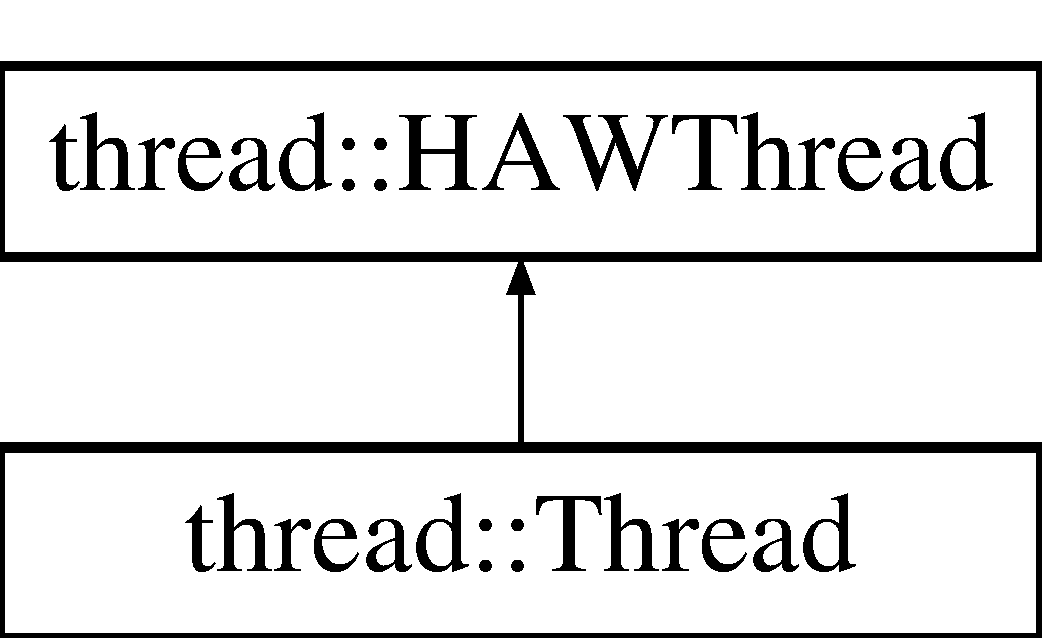
\includegraphics[height=2.000000cm]{classthread_1_1_h_a_w_thread}
\end{center}
\end{figure}
\subsection*{Public Member Functions}
\begin{DoxyCompactItemize}
\item 
\hyperlink{classthread_1_1_h_a_w_thread_a7ae3280c8aee6ae6536c736a20d92e8d}{H\-A\-W\-Thread} ()
\item 
virtual \hyperlink{classthread_1_1_h_a_w_thread_a84706dda23aa384a43ced901381e795b}{$\sim$\-H\-A\-W\-Thread} ()
\item 
void \hyperlink{classthread_1_1_h_a_w_thread_ae08d268c337511a1e67fbbeefcb1e89d}{start} (void $\ast$arg)
\item 
void \hyperlink{classthread_1_1_h_a_w_thread_ae8a89c83fd7e9b9a712c19f636ab2638}{stop} ()
\item 
void \hyperlink{classthread_1_1_h_a_w_thread_a4732efa3445c499f1723971acc07863f}{join} () const 
\item 
void \hyperlink{classthread_1_1_h_a_w_thread_a18f2a0cc61833e98b18e56ea541fa38b}{hold} ()
\item 
void \hyperlink{classthread_1_1_h_a_w_thread_a4c480261e3236c90c8de73be55650ba4}{cont} ()
\end{DoxyCompactItemize}
\subsection*{Protected Member Functions}
\begin{DoxyCompactItemize}
\item 
void \hyperlink{classthread_1_1_h_a_w_thread_a9a3e17be59877d350e310eb19c52679b}{run} (void $\ast$arg)
\item 
virtual void \hyperlink{classthread_1_1_h_a_w_thread_ae565cb73c096b246664bd2474b9c8907}{execute} (void $\ast$)=0
\item 
virtual void \hyperlink{classthread_1_1_h_a_w_thread_a843ee9493a41cec7e932fdec67a3b244}{shutdown} ()=0
\item 
void $\ast$ \hyperlink{classthread_1_1_h_a_w_thread_ab692f3a55b92623653d8213793ba4ebb}{Arg} () const 
\item 
void \hyperlink{classthread_1_1_h_a_w_thread_a368c07a801fb8f5e7bb181d2453df4be}{Arg} (void $\ast$a)
\item 
bool \hyperlink{classthread_1_1_h_a_w_thread_a46e9f127856f36917b3a8a345b7be5ee}{is\-Stopped} () const 
\item 
void \hyperlink{classthread_1_1_h_a_w_thread_a5124385e940aa8d52510a4be10af173c}{shutdown\-All} ()
\end{DoxyCompactItemize}
\subsection*{Static Protected Member Functions}
\begin{DoxyCompactItemize}
\item 
static void $\ast$ \hyperlink{classthread_1_1_h_a_w_thread_a044da2e1a8884a3e2764f9f1863863c7}{entry\-Point} (void $\ast$)
\end{DoxyCompactItemize}


\subsection{Constructor \& Destructor Documentation}
\hypertarget{classthread_1_1_h_a_w_thread_a7ae3280c8aee6ae6536c736a20d92e8d}{\index{thread\-::\-H\-A\-W\-Thread@{thread\-::\-H\-A\-W\-Thread}!H\-A\-W\-Thread@{H\-A\-W\-Thread}}
\index{H\-A\-W\-Thread@{H\-A\-W\-Thread}!thread::HAWThread@{thread\-::\-H\-A\-W\-Thread}}
\subsubsection[{H\-A\-W\-Thread}]{\setlength{\rightskip}{0pt plus 5cm}thread\-::\-H\-A\-W\-Thread\-::\-H\-A\-W\-Thread (
\begin{DoxyParamCaption}
{}
\end{DoxyParamCaption}
)}}\label{classthread_1_1_h_a_w_thread_a7ae3280c8aee6ae6536c736a20d92e8d}
Constructor. Initializes members \hypertarget{classthread_1_1_h_a_w_thread_a84706dda23aa384a43ced901381e795b}{\index{thread\-::\-H\-A\-W\-Thread@{thread\-::\-H\-A\-W\-Thread}!$\sim$\-H\-A\-W\-Thread@{$\sim$\-H\-A\-W\-Thread}}
\index{$\sim$\-H\-A\-W\-Thread@{$\sim$\-H\-A\-W\-Thread}!thread::HAWThread@{thread\-::\-H\-A\-W\-Thread}}
\subsubsection[{$\sim$\-H\-A\-W\-Thread}]{\setlength{\rightskip}{0pt plus 5cm}thread\-::\-H\-A\-W\-Thread\-::$\sim$\-H\-A\-W\-Thread (
\begin{DoxyParamCaption}
{}
\end{DoxyParamCaption}
)\hspace{0.3cm}{\ttfamily [virtual]}}}\label{classthread_1_1_h_a_w_thread_a84706dda23aa384a43ced901381e795b}
Destructor. Calls Thread\-Destroy. This should shutdown the thread more carefully. \begin{DoxyWarning}{Warning}
needs some work! 
\end{DoxyWarning}


\subsection{Member Function Documentation}
\hypertarget{classthread_1_1_h_a_w_thread_ab692f3a55b92623653d8213793ba4ebb}{\index{thread\-::\-H\-A\-W\-Thread@{thread\-::\-H\-A\-W\-Thread}!Arg@{Arg}}
\index{Arg@{Arg}!thread::HAWThread@{thread\-::\-H\-A\-W\-Thread}}
\subsubsection[{Arg}]{\setlength{\rightskip}{0pt plus 5cm}void$\ast$ thread\-::\-H\-A\-W\-Thread\-::\-Arg (
\begin{DoxyParamCaption}
{}
\end{DoxyParamCaption}
) const\hspace{0.3cm}{\ttfamily [inline]}, {\ttfamily [protected]}}}\label{classthread_1_1_h_a_w_thread_ab692f3a55b92623653d8213793ba4ebb}
used internally to pass the argument. \hypertarget{classthread_1_1_h_a_w_thread_a368c07a801fb8f5e7bb181d2453df4be}{\index{thread\-::\-H\-A\-W\-Thread@{thread\-::\-H\-A\-W\-Thread}!Arg@{Arg}}
\index{Arg@{Arg}!thread::HAWThread@{thread\-::\-H\-A\-W\-Thread}}
\subsubsection[{Arg}]{\setlength{\rightskip}{0pt plus 5cm}void thread\-::\-H\-A\-W\-Thread\-::\-Arg (
\begin{DoxyParamCaption}
\item[{void $\ast$}]{a}
\end{DoxyParamCaption}
)\hspace{0.3cm}{\ttfamily [inline]}, {\ttfamily [protected]}}}\label{classthread_1_1_h_a_w_thread_a368c07a801fb8f5e7bb181d2453df4be}
used internally to set the arguement. \hypertarget{classthread_1_1_h_a_w_thread_a4c480261e3236c90c8de73be55650ba4}{\index{thread\-::\-H\-A\-W\-Thread@{thread\-::\-H\-A\-W\-Thread}!cont@{cont}}
\index{cont@{cont}!thread::HAWThread@{thread\-::\-H\-A\-W\-Thread}}
\subsubsection[{cont}]{\setlength{\rightskip}{0pt plus 5cm}void thread\-::\-H\-A\-W\-Thread\-::cont (
\begin{DoxyParamCaption}
{}
\end{DoxyParamCaption}
)}}\label{classthread_1_1_h_a_w_thread_a4c480261e3236c90c8de73be55650ba4}
This function continues (resumes) the thread. It makes a Thread\-Ctrl call. \hypertarget{classthread_1_1_h_a_w_thread_a044da2e1a8884a3e2764f9f1863863c7}{\index{thread\-::\-H\-A\-W\-Thread@{thread\-::\-H\-A\-W\-Thread}!entry\-Point@{entry\-Point}}
\index{entry\-Point@{entry\-Point}!thread::HAWThread@{thread\-::\-H\-A\-W\-Thread}}
\subsubsection[{entry\-Point}]{\setlength{\rightskip}{0pt plus 5cm}void $\ast$ thread\-::\-H\-A\-W\-Thread\-::entry\-Point (
\begin{DoxyParamCaption}
\item[{void $\ast$}]{pthis}
\end{DoxyParamCaption}
)\hspace{0.3cm}{\ttfamily [static]}, {\ttfamily [protected]}}}\label{classthread_1_1_h_a_w_thread_a044da2e1a8884a3e2764f9f1863863c7}
\hypertarget{classthread_1_1_h_a_w_thread_ae565cb73c096b246664bd2474b9c8907}{\index{thread\-::\-H\-A\-W\-Thread@{thread\-::\-H\-A\-W\-Thread}!execute@{execute}}
\index{execute@{execute}!thread::HAWThread@{thread\-::\-H\-A\-W\-Thread}}
\subsubsection[{execute}]{\setlength{\rightskip}{0pt plus 5cm}virtual void thread\-::\-H\-A\-W\-Thread\-::execute (
\begin{DoxyParamCaption}
\item[{void $\ast$}]{}
\end{DoxyParamCaption}
)\hspace{0.3cm}{\ttfamily [protected]}, {\ttfamily [pure virtual]}}}\label{classthread_1_1_h_a_w_thread_ae565cb73c096b246664bd2474b9c8907}
to be implemented in the derived class. The application programmer has to write his own loop. He can check bool \hyperlink{classthread_1_1_h_a_w_thread_a46e9f127856f36917b3a8a345b7be5ee}{is\-Stopped()} to see if the thread should exit the loop. 

Implemented in \hyperlink{classthread_1_1_thread_a2444c1af4f269dacaead0ec8ee266123}{thread\-::\-Thread}.

\hypertarget{classthread_1_1_h_a_w_thread_a18f2a0cc61833e98b18e56ea541fa38b}{\index{thread\-::\-H\-A\-W\-Thread@{thread\-::\-H\-A\-W\-Thread}!hold@{hold}}
\index{hold@{hold}!thread::HAWThread@{thread\-::\-H\-A\-W\-Thread}}
\subsubsection[{hold}]{\setlength{\rightskip}{0pt plus 5cm}void thread\-::\-H\-A\-W\-Thread\-::hold (
\begin{DoxyParamCaption}
{}
\end{DoxyParamCaption}
)}}\label{classthread_1_1_h_a_w_thread_a18f2a0cc61833e98b18e56ea541fa38b}
This function holds (suspends) the thread. It makes a Thread\-Ctrl call. It shall be used if the thread is not being used for a while but may be used later \hypertarget{classthread_1_1_h_a_w_thread_a46e9f127856f36917b3a8a345b7be5ee}{\index{thread\-::\-H\-A\-W\-Thread@{thread\-::\-H\-A\-W\-Thread}!is\-Stopped@{is\-Stopped}}
\index{is\-Stopped@{is\-Stopped}!thread::HAWThread@{thread\-::\-H\-A\-W\-Thread}}
\subsubsection[{is\-Stopped}]{\setlength{\rightskip}{0pt plus 5cm}bool thread\-::\-H\-A\-W\-Thread\-::is\-Stopped (
\begin{DoxyParamCaption}
{}
\end{DoxyParamCaption}
) const\hspace{0.3cm}{\ttfamily [inline]}, {\ttfamily [protected]}}}\label{classthread_1_1_h_a_w_thread_a46e9f127856f36917b3a8a345b7be5ee}
returns the stop-\/status of the thread. This function should be checked by the user function execute regularly. \hypertarget{classthread_1_1_h_a_w_thread_a4732efa3445c499f1723971acc07863f}{\index{thread\-::\-H\-A\-W\-Thread@{thread\-::\-H\-A\-W\-Thread}!join@{join}}
\index{join@{join}!thread::HAWThread@{thread\-::\-H\-A\-W\-Thread}}
\subsubsection[{join}]{\setlength{\rightskip}{0pt plus 5cm}void thread\-::\-H\-A\-W\-Thread\-::join (
\begin{DoxyParamCaption}
{}
\end{DoxyParamCaption}
) const}}\label{classthread_1_1_h_a_w_thread_a4732efa3445c499f1723971acc07863f}
Calls join on the thread. \begin{DoxyWarning}{Warning}
must be called from the same context as start. 
\end{DoxyWarning}
\hypertarget{classthread_1_1_h_a_w_thread_a9a3e17be59877d350e310eb19c52679b}{\index{thread\-::\-H\-A\-W\-Thread@{thread\-::\-H\-A\-W\-Thread}!run@{run}}
\index{run@{run}!thread::HAWThread@{thread\-::\-H\-A\-W\-Thread}}
\subsubsection[{run}]{\setlength{\rightskip}{0pt plus 5cm}void thread\-::\-H\-A\-W\-Thread\-::run (
\begin{DoxyParamCaption}
\item[{void $\ast$}]{arg}
\end{DoxyParamCaption}
)\hspace{0.3cm}{\ttfamily [protected]}}}\label{classthread_1_1_h_a_w_thread_a9a3e17be59877d350e310eb19c52679b}
This is called when the thread is started. It calls execute an shutdown which are the user functions. \hypertarget{classthread_1_1_h_a_w_thread_a843ee9493a41cec7e932fdec67a3b244}{\index{thread\-::\-H\-A\-W\-Thread@{thread\-::\-H\-A\-W\-Thread}!shutdown@{shutdown}}
\index{shutdown@{shutdown}!thread::HAWThread@{thread\-::\-H\-A\-W\-Thread}}
\subsubsection[{shutdown}]{\setlength{\rightskip}{0pt plus 5cm}virtual void thread\-::\-H\-A\-W\-Thread\-::shutdown (
\begin{DoxyParamCaption}
{}
\end{DoxyParamCaption}
)\hspace{0.3cm}{\ttfamily [protected]}, {\ttfamily [pure virtual]}}}\label{classthread_1_1_h_a_w_thread_a843ee9493a41cec7e932fdec67a3b244}
this function must be implemented in the derived class. The function is called once after the thread has been stopped. 

Implemented in \hyperlink{classthread_1_1_thread_abda49d1f648def9611927897cbae668d}{thread\-::\-Thread}.

\hypertarget{classthread_1_1_h_a_w_thread_a5124385e940aa8d52510a4be10af173c}{\index{thread\-::\-H\-A\-W\-Thread@{thread\-::\-H\-A\-W\-Thread}!shutdown\-All@{shutdown\-All}}
\index{shutdown\-All@{shutdown\-All}!thread::HAWThread@{thread\-::\-H\-A\-W\-Thread}}
\subsubsection[{shutdown\-All}]{\setlength{\rightskip}{0pt plus 5cm}void thread\-::\-H\-A\-W\-Thread\-::shutdown\-All (
\begin{DoxyParamCaption}
{}
\end{DoxyParamCaption}
)\hspace{0.3cm}{\ttfamily [inline]}, {\ttfamily [protected]}}}\label{classthread_1_1_h_a_w_thread_a5124385e940aa8d52510a4be10af173c}
sets the G\-L\-O\-B\-A\-L\-\_\-\-E\-X\-I\-T flag to true. \hypertarget{classthread_1_1_h_a_w_thread_ae08d268c337511a1e67fbbeefcb1e89d}{\index{thread\-::\-H\-A\-W\-Thread@{thread\-::\-H\-A\-W\-Thread}!start@{start}}
\index{start@{start}!thread::HAWThread@{thread\-::\-H\-A\-W\-Thread}}
\subsubsection[{start}]{\setlength{\rightskip}{0pt plus 5cm}void thread\-::\-H\-A\-W\-Thread\-::start (
\begin{DoxyParamCaption}
\item[{void $\ast$}]{arg}
\end{DoxyParamCaption}
)}}\label{classthread_1_1_h_a_w_thread_ae08d268c337511a1e67fbbeefcb1e89d}
Starts the \hyperlink{classthread_1_1_thread}{Thread}. \begin{DoxyWarning}{Warning}
start must be called always from the same context as \hyperlink{classthread_1_1_h_a_w_thread_ae8a89c83fd7e9b9a712c19f636ab2638}{stop()}. 

If \hyperlink{classthread_1_1_thread}{Thread} is already running, \hyperlink{classthread_1_1_h_a_w_thread_ae08d268c337511a1e67fbbeefcb1e89d}{start()} is a N\-O\-P. \begin{DoxyItemize}
\item argument is stored locally as a member. \end{DoxyItemize}

\end{DoxyWarning}
\hypertarget{classthread_1_1_h_a_w_thread_ae8a89c83fd7e9b9a712c19f636ab2638}{\index{thread\-::\-H\-A\-W\-Thread@{thread\-::\-H\-A\-W\-Thread}!stop@{stop}}
\index{stop@{stop}!thread::HAWThread@{thread\-::\-H\-A\-W\-Thread}}
\subsubsection[{stop}]{\setlength{\rightskip}{0pt plus 5cm}void thread\-::\-H\-A\-W\-Thread\-::stop (
\begin{DoxyParamCaption}
{}
\end{DoxyParamCaption}
)}}\label{classthread_1_1_h_a_w_thread_ae8a89c83fd7e9b9a712c19f636ab2638}
Sets the internal flag L\-O\-C\-A\-L\-\_\-\-E\-X\-I\-T to true. 

The documentation for this class was generated from the following files\-:\begin{DoxyCompactItemize}
\item 
Software/\-S\-E2\-P2/\-H\-A\-W/\hyperlink{_h_a_w_thread_8h}{H\-A\-W\-Thread.\-h}\item 
Software/\-S\-E2\-P2/\-H\-A\-W/\hyperlink{_h_a_w_thread_8cpp}{H\-A\-W\-Thread.\-cpp}\end{DoxyCompactItemize}

\hypertarget{class_mutex}{\section{Mutex Class Reference}
\label{class_mutex}\index{Mutex@{Mutex}}
}


{\ttfamily \#include $<$Mutex.\-h$>$}

\subsection*{Public Member Functions}
\begin{DoxyCompactItemize}
\item 
\hyperlink{class_mutex_a593423d868daf926c7b0d63a833ae29a}{Mutex} ()
\item 
\hyperlink{class_mutex_ac9e9182407f5f74892318607888e9be4}{$\sim$\-Mutex} ()
\item 
void \hyperlink{class_mutex_ad91be808bf0a60a16f10b897ec246d3a}{lock} ()
\item 
void \hyperlink{class_mutex_a546a5b797ba29959357586aa2b3740a8}{unlock} ()
\end{DoxyCompactItemize}


\subsection{Detailed Description}


Definition at line 12 of file Mutex.\-h.



\subsection{Constructor \& Destructor Documentation}
\hypertarget{class_mutex_a593423d868daf926c7b0d63a833ae29a}{\index{Mutex@{Mutex}!Mutex@{Mutex}}
\index{Mutex@{Mutex}!Mutex@{Mutex}}
\subsubsection[{Mutex}]{\setlength{\rightskip}{0pt plus 5cm}Mutex\-::\-Mutex (
\begin{DoxyParamCaption}
{}
\end{DoxyParamCaption}
)}}\label{class_mutex_a593423d868daf926c7b0d63a833ae29a}


Definition at line 16 of file Mutex.\-cpp.

\hypertarget{class_mutex_ac9e9182407f5f74892318607888e9be4}{\index{Mutex@{Mutex}!$\sim$\-Mutex@{$\sim$\-Mutex}}
\index{$\sim$\-Mutex@{$\sim$\-Mutex}!Mutex@{Mutex}}
\subsubsection[{$\sim$\-Mutex}]{\setlength{\rightskip}{0pt plus 5cm}Mutex\-::$\sim$\-Mutex (
\begin{DoxyParamCaption}
{}
\end{DoxyParamCaption}
)}}\label{class_mutex_ac9e9182407f5f74892318607888e9be4}


Definition at line 23 of file Mutex.\-cpp.



\subsection{Member Function Documentation}
\hypertarget{class_mutex_ad91be808bf0a60a16f10b897ec246d3a}{\index{Mutex@{Mutex}!lock@{lock}}
\index{lock@{lock}!Mutex@{Mutex}}
\subsubsection[{lock}]{\setlength{\rightskip}{0pt plus 5cm}void Mutex\-::lock (
\begin{DoxyParamCaption}
{}
\end{DoxyParamCaption}
)}}\label{class_mutex_ad91be808bf0a60a16f10b897ec246d3a}


Definition at line 30 of file Mutex.\-cpp.

\hypertarget{class_mutex_a546a5b797ba29959357586aa2b3740a8}{\index{Mutex@{Mutex}!unlock@{unlock}}
\index{unlock@{unlock}!Mutex@{Mutex}}
\subsubsection[{unlock}]{\setlength{\rightskip}{0pt plus 5cm}void Mutex\-::unlock (
\begin{DoxyParamCaption}
{}
\end{DoxyParamCaption}
)}}\label{class_mutex_a546a5b797ba29959357586aa2b3740a8}


Definition at line 37 of file Mutex.\-cpp.



The documentation for this class was generated from the following files\-:\begin{DoxyCompactItemize}
\item 
C\-:/\-Users/\-Nata/\-Documents/\-S\-E\-P2/sourcetree/\-Software/\-S\-E2\-P2/\-Mutex/\hyperlink{_mutex_8h}{Mutex.\-h}\item 
C\-:/\-Users/\-Nata/\-Documents/\-S\-E\-P2/sourcetree/\-Software/\-S\-E2\-P2/\-Mutex/\hyperlink{_mutex_8cpp}{Mutex.\-cpp}\end{DoxyCompactItemize}

\hypertarget{classthread_1_1_thread}{\section{thread\-:\-:Thread Class Reference}
\label{classthread_1_1_thread}\index{thread\-::\-Thread@{thread\-::\-Thread}}
}


{\ttfamily \#include $<$Thread.\-h$>$}

Inheritance diagram for thread\-:\-:Thread\-:\begin{figure}[H]
\begin{center}
\leavevmode
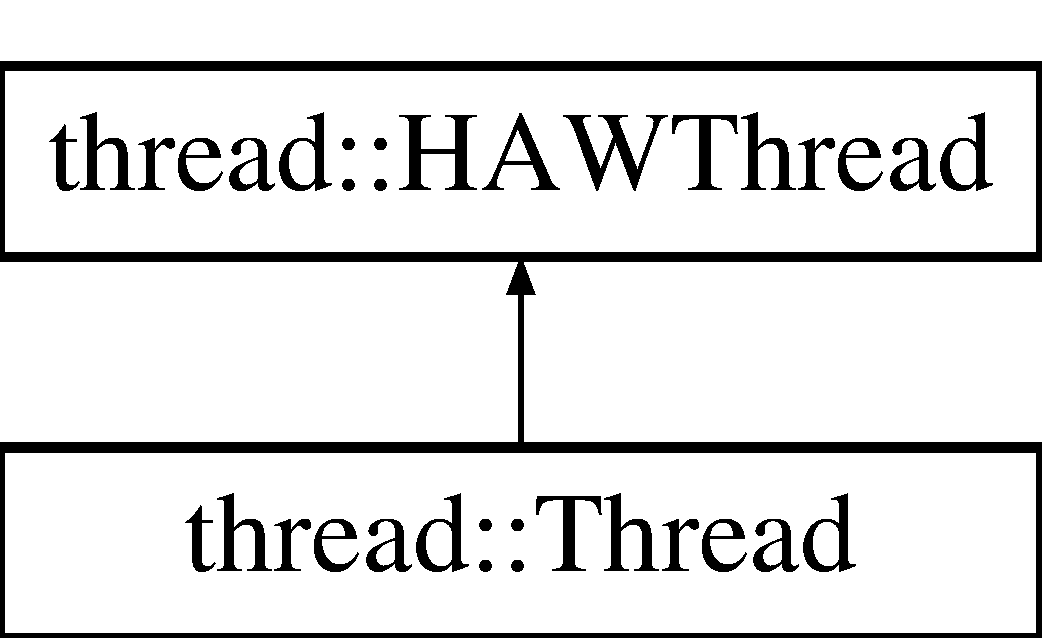
\includegraphics[height=2.000000cm]{classthread_1_1_thread}
\end{center}
\end{figure}
\subsection*{Public Member Functions}
\begin{DoxyCompactItemize}
\item 
\hyperlink{classthread_1_1_thread_ade4761946b42cc3d1a32fc04f5405f48}{Thread} ()
\item 
virtual \hyperlink{classthread_1_1_thread_a5cc06f9b6a7fe494e0f64e4476117255}{$\sim$\-Thread} ()
\item 
virtual void \hyperlink{classthread_1_1_thread_a2444c1af4f269dacaead0ec8ee266123}{execute} (void $\ast$arg)
\item 
virtual void \hyperlink{classthread_1_1_thread_abda49d1f648def9611927897cbae668d}{shutdown} ()
\end{DoxyCompactItemize}
\subsection*{Additional Inherited Members}


\subsection{Detailed Description}


Definition at line 21 of file Thread.\-h.



\subsection{Constructor \& Destructor Documentation}
\hypertarget{classthread_1_1_thread_ade4761946b42cc3d1a32fc04f5405f48}{\index{thread\-::\-Thread@{thread\-::\-Thread}!Thread@{Thread}}
\index{Thread@{Thread}!thread::Thread@{thread\-::\-Thread}}
\subsubsection[{Thread}]{\setlength{\rightskip}{0pt plus 5cm}thread\-::\-Thread\-::\-Thread (
\begin{DoxyParamCaption}
{}
\end{DoxyParamCaption}
)}}\label{classthread_1_1_thread_ade4761946b42cc3d1a32fc04f5405f48}


Definition at line 22 of file Thread.\-cpp.

\hypertarget{classthread_1_1_thread_a5cc06f9b6a7fe494e0f64e4476117255}{\index{thread\-::\-Thread@{thread\-::\-Thread}!$\sim$\-Thread@{$\sim$\-Thread}}
\index{$\sim$\-Thread@{$\sim$\-Thread}!thread::Thread@{thread\-::\-Thread}}
\subsubsection[{$\sim$\-Thread}]{\setlength{\rightskip}{0pt plus 5cm}thread\-::\-Thread\-::$\sim$\-Thread (
\begin{DoxyParamCaption}
{}
\end{DoxyParamCaption}
)\hspace{0.3cm}{\ttfamily [virtual]}}}\label{classthread_1_1_thread_a5cc06f9b6a7fe494e0f64e4476117255}


Definition at line 28 of file Thread.\-cpp.



\subsection{Member Function Documentation}
\hypertarget{classthread_1_1_thread_a2444c1af4f269dacaead0ec8ee266123}{\index{thread\-::\-Thread@{thread\-::\-Thread}!execute@{execute}}
\index{execute@{execute}!thread::Thread@{thread\-::\-Thread}}
\subsubsection[{execute}]{\setlength{\rightskip}{0pt plus 5cm}void thread\-::\-Thread\-::execute (
\begin{DoxyParamCaption}
\item[{void $\ast$}]{}
\end{DoxyParamCaption}
)\hspace{0.3cm}{\ttfamily [virtual]}}}\label{classthread_1_1_thread_a2444c1af4f269dacaead0ec8ee266123}
to be implemented in the derived class. The application programmer has to write his own loop. He can check bool \hyperlink{classthread_1_1_h_a_w_thread_a46e9f127856f36917b3a8a345b7be5ee}{is\-Stopped()} to see if the thread should exit the loop. 

Implements \hyperlink{classthread_1_1_h_a_w_thread_ae565cb73c096b246664bd2474b9c8907}{thread\-::\-H\-A\-W\-Thread}.



Definition at line 39 of file Thread.\-cpp.

\hypertarget{classthread_1_1_thread_abda49d1f648def9611927897cbae668d}{\index{thread\-::\-Thread@{thread\-::\-Thread}!shutdown@{shutdown}}
\index{shutdown@{shutdown}!thread::Thread@{thread\-::\-Thread}}
\subsubsection[{shutdown}]{\setlength{\rightskip}{0pt plus 5cm}void thread\-::\-Thread\-::shutdown (
\begin{DoxyParamCaption}
{}
\end{DoxyParamCaption}
)\hspace{0.3cm}{\ttfamily [virtual]}}}\label{classthread_1_1_thread_abda49d1f648def9611927897cbae668d}
this function must be implemented in the derived class. The function is called once after the thread has been stopped. 

Implements \hyperlink{classthread_1_1_h_a_w_thread_a843ee9493a41cec7e932fdec67a3b244}{thread\-::\-H\-A\-W\-Thread}.



Definition at line 32 of file Thread.\-cpp.



The documentation for this class was generated from the following files\-:\begin{DoxyCompactItemize}
\item 
C\-:/\-Users/\-Nata/\-Documents/\-S\-E\-P2/sourcetree/\-Software/\-S\-E2\-P2/\hyperlink{_thread_8h}{Thread.\-h}\item 
C\-:/\-Users/\-Nata/\-Documents/\-S\-E\-P2/sourcetree/\-Software/\-S\-E2\-P2/\hyperlink{_thread_8cpp}{Thread.\-cpp}\end{DoxyCompactItemize}

\chapter{File Documentation}
\hypertarget{_r_e_a_d_m_e_8md}{\section{R\-E\-A\-D\-M\-E.\-md File Reference}
\label{_r_e_a_d_m_e_8md}\index{R\-E\-A\-D\-M\-E.\-md@{R\-E\-A\-D\-M\-E.\-md}}
}

\hypertarget{_addresses_8h}{\section{Software/\-S\-E2\-P2/\-H\-A\-L/\-Addresses.h File Reference}
\label{_addresses_8h}\index{Software/\-S\-E2\-P2/\-H\-A\-L/\-Addresses.\-h@{Software/\-S\-E2\-P2/\-H\-A\-L/\-Addresses.\-h}}
}
\subsection*{Macros}
\begin{DoxyCompactItemize}
\item 
\#define \hyperlink{_addresses_8h_a57314fe3306fd02b396aedcdc58749ec}{D\-I\-O\-\_\-\-B\-A\-S\-E}~0x300
\item 
\#define \hyperlink{_addresses_8h_a75c06dd12f0060ca328bf82ba2103ec2}{D\-I\-O\-\_\-\-O\-F\-F\-S\-\_\-\-A}~0x00
\item 
\#define \hyperlink{_addresses_8h_abc7b19477102fe9e63b88c77b0c16e24}{D\-I\-O\-\_\-\-O\-F\-F\-S\-\_\-\-B}~0x01
\item 
\#define \hyperlink{_addresses_8h_a186d39b18319d4f9f9f500228760f89a}{D\-I\-O\-\_\-\-O\-F\-F\-S\-\_\-\-C}~0x02
\item 
\#define \hyperlink{_addresses_8h_a30bfb5a58855ac19adc4c8dba22a7d38}{D\-I\-O\-\_\-\-O\-F\-F\-S\-\_\-\-C\-T\-R\-L}~0x03
\item 
\#define \hyperlink{_addresses_8h_add6d2693f5d356b091088437148f939b}{B\-I\-T\-\_\-0}~0x01
\item 
\#define \hyperlink{_addresses_8h_aec9fa7211b7c9a686f2cd522cad7989d}{B\-I\-T\-\_\-1}~0x02
\item 
\#define \hyperlink{_addresses_8h_ab94e068b5073d729aad6b2aeb613916c}{B\-I\-T\-\_\-2}~0x04
\item 
\#define \hyperlink{_addresses_8h_a2cad0186598ab53983a3bca9b09b0a51}{B\-I\-T\-\_\-3}~0x08
\item 
\#define \hyperlink{_addresses_8h_a3506434dff748a6be0d75a338a95e673}{B\-I\-T\-\_\-4}~0x10
\item 
\#define \hyperlink{_addresses_8h_aae7fda97814f05bfe68c0f6bb2ef9f11}{B\-I\-T\-\_\-5}~0x20
\item 
\#define \hyperlink{_addresses_8h_a7ecb78fe8c01d9722a06f10691495309}{B\-I\-T\-\_\-6}~0x40
\item 
\#define \hyperlink{_addresses_8h_a4ad58adf84157aebea2a98cc9402212a}{B\-I\-T\-\_\-7}~0x80
\end{DoxyCompactItemize}


\subsection{Macro Definition Documentation}
\hypertarget{_addresses_8h_add6d2693f5d356b091088437148f939b}{\index{Addresses.\-h@{Addresses.\-h}!B\-I\-T\-\_\-0@{B\-I\-T\-\_\-0}}
\index{B\-I\-T\-\_\-0@{B\-I\-T\-\_\-0}!Addresses.h@{Addresses.\-h}}
\subsubsection[{B\-I\-T\-\_\-0}]{\setlength{\rightskip}{0pt plus 5cm}\#define B\-I\-T\-\_\-0~0x01}}\label{_addresses_8h_add6d2693f5d356b091088437148f939b}
\hypertarget{_addresses_8h_aec9fa7211b7c9a686f2cd522cad7989d}{\index{Addresses.\-h@{Addresses.\-h}!B\-I\-T\-\_\-1@{B\-I\-T\-\_\-1}}
\index{B\-I\-T\-\_\-1@{B\-I\-T\-\_\-1}!Addresses.h@{Addresses.\-h}}
\subsubsection[{B\-I\-T\-\_\-1}]{\setlength{\rightskip}{0pt plus 5cm}\#define B\-I\-T\-\_\-1~0x02}}\label{_addresses_8h_aec9fa7211b7c9a686f2cd522cad7989d}
\hypertarget{_addresses_8h_ab94e068b5073d729aad6b2aeb613916c}{\index{Addresses.\-h@{Addresses.\-h}!B\-I\-T\-\_\-2@{B\-I\-T\-\_\-2}}
\index{B\-I\-T\-\_\-2@{B\-I\-T\-\_\-2}!Addresses.h@{Addresses.\-h}}
\subsubsection[{B\-I\-T\-\_\-2}]{\setlength{\rightskip}{0pt plus 5cm}\#define B\-I\-T\-\_\-2~0x04}}\label{_addresses_8h_ab94e068b5073d729aad6b2aeb613916c}
\hypertarget{_addresses_8h_a2cad0186598ab53983a3bca9b09b0a51}{\index{Addresses.\-h@{Addresses.\-h}!B\-I\-T\-\_\-3@{B\-I\-T\-\_\-3}}
\index{B\-I\-T\-\_\-3@{B\-I\-T\-\_\-3}!Addresses.h@{Addresses.\-h}}
\subsubsection[{B\-I\-T\-\_\-3}]{\setlength{\rightskip}{0pt plus 5cm}\#define B\-I\-T\-\_\-3~0x08}}\label{_addresses_8h_a2cad0186598ab53983a3bca9b09b0a51}
\hypertarget{_addresses_8h_a3506434dff748a6be0d75a338a95e673}{\index{Addresses.\-h@{Addresses.\-h}!B\-I\-T\-\_\-4@{B\-I\-T\-\_\-4}}
\index{B\-I\-T\-\_\-4@{B\-I\-T\-\_\-4}!Addresses.h@{Addresses.\-h}}
\subsubsection[{B\-I\-T\-\_\-4}]{\setlength{\rightskip}{0pt plus 5cm}\#define B\-I\-T\-\_\-4~0x10}}\label{_addresses_8h_a3506434dff748a6be0d75a338a95e673}
\hypertarget{_addresses_8h_aae7fda97814f05bfe68c0f6bb2ef9f11}{\index{Addresses.\-h@{Addresses.\-h}!B\-I\-T\-\_\-5@{B\-I\-T\-\_\-5}}
\index{B\-I\-T\-\_\-5@{B\-I\-T\-\_\-5}!Addresses.h@{Addresses.\-h}}
\subsubsection[{B\-I\-T\-\_\-5}]{\setlength{\rightskip}{0pt plus 5cm}\#define B\-I\-T\-\_\-5~0x20}}\label{_addresses_8h_aae7fda97814f05bfe68c0f6bb2ef9f11}
\hypertarget{_addresses_8h_a7ecb78fe8c01d9722a06f10691495309}{\index{Addresses.\-h@{Addresses.\-h}!B\-I\-T\-\_\-6@{B\-I\-T\-\_\-6}}
\index{B\-I\-T\-\_\-6@{B\-I\-T\-\_\-6}!Addresses.h@{Addresses.\-h}}
\subsubsection[{B\-I\-T\-\_\-6}]{\setlength{\rightskip}{0pt plus 5cm}\#define B\-I\-T\-\_\-6~0x40}}\label{_addresses_8h_a7ecb78fe8c01d9722a06f10691495309}
\hypertarget{_addresses_8h_a4ad58adf84157aebea2a98cc9402212a}{\index{Addresses.\-h@{Addresses.\-h}!B\-I\-T\-\_\-7@{B\-I\-T\-\_\-7}}
\index{B\-I\-T\-\_\-7@{B\-I\-T\-\_\-7}!Addresses.h@{Addresses.\-h}}
\subsubsection[{B\-I\-T\-\_\-7}]{\setlength{\rightskip}{0pt plus 5cm}\#define B\-I\-T\-\_\-7~0x80}}\label{_addresses_8h_a4ad58adf84157aebea2a98cc9402212a}
\hypertarget{_addresses_8h_a57314fe3306fd02b396aedcdc58749ec}{\index{Addresses.\-h@{Addresses.\-h}!D\-I\-O\-\_\-\-B\-A\-S\-E@{D\-I\-O\-\_\-\-B\-A\-S\-E}}
\index{D\-I\-O\-\_\-\-B\-A\-S\-E@{D\-I\-O\-\_\-\-B\-A\-S\-E}!Addresses.h@{Addresses.\-h}}
\subsubsection[{D\-I\-O\-\_\-\-B\-A\-S\-E}]{\setlength{\rightskip}{0pt plus 5cm}\#define D\-I\-O\-\_\-\-B\-A\-S\-E~0x300}}\label{_addresses_8h_a57314fe3306fd02b396aedcdc58749ec}
\hypertarget{_addresses_8h_a75c06dd12f0060ca328bf82ba2103ec2}{\index{Addresses.\-h@{Addresses.\-h}!D\-I\-O\-\_\-\-O\-F\-F\-S\-\_\-\-A@{D\-I\-O\-\_\-\-O\-F\-F\-S\-\_\-\-A}}
\index{D\-I\-O\-\_\-\-O\-F\-F\-S\-\_\-\-A@{D\-I\-O\-\_\-\-O\-F\-F\-S\-\_\-\-A}!Addresses.h@{Addresses.\-h}}
\subsubsection[{D\-I\-O\-\_\-\-O\-F\-F\-S\-\_\-\-A}]{\setlength{\rightskip}{0pt plus 5cm}\#define D\-I\-O\-\_\-\-O\-F\-F\-S\-\_\-\-A~0x00}}\label{_addresses_8h_a75c06dd12f0060ca328bf82ba2103ec2}
\hypertarget{_addresses_8h_abc7b19477102fe9e63b88c77b0c16e24}{\index{Addresses.\-h@{Addresses.\-h}!D\-I\-O\-\_\-\-O\-F\-F\-S\-\_\-\-B@{D\-I\-O\-\_\-\-O\-F\-F\-S\-\_\-\-B}}
\index{D\-I\-O\-\_\-\-O\-F\-F\-S\-\_\-\-B@{D\-I\-O\-\_\-\-O\-F\-F\-S\-\_\-\-B}!Addresses.h@{Addresses.\-h}}
\subsubsection[{D\-I\-O\-\_\-\-O\-F\-F\-S\-\_\-\-B}]{\setlength{\rightskip}{0pt plus 5cm}\#define D\-I\-O\-\_\-\-O\-F\-F\-S\-\_\-\-B~0x01}}\label{_addresses_8h_abc7b19477102fe9e63b88c77b0c16e24}
\hypertarget{_addresses_8h_a186d39b18319d4f9f9f500228760f89a}{\index{Addresses.\-h@{Addresses.\-h}!D\-I\-O\-\_\-\-O\-F\-F\-S\-\_\-\-C@{D\-I\-O\-\_\-\-O\-F\-F\-S\-\_\-\-C}}
\index{D\-I\-O\-\_\-\-O\-F\-F\-S\-\_\-\-C@{D\-I\-O\-\_\-\-O\-F\-F\-S\-\_\-\-C}!Addresses.h@{Addresses.\-h}}
\subsubsection[{D\-I\-O\-\_\-\-O\-F\-F\-S\-\_\-\-C}]{\setlength{\rightskip}{0pt plus 5cm}\#define D\-I\-O\-\_\-\-O\-F\-F\-S\-\_\-\-C~0x02}}\label{_addresses_8h_a186d39b18319d4f9f9f500228760f89a}
\hypertarget{_addresses_8h_a30bfb5a58855ac19adc4c8dba22a7d38}{\index{Addresses.\-h@{Addresses.\-h}!D\-I\-O\-\_\-\-O\-F\-F\-S\-\_\-\-C\-T\-R\-L@{D\-I\-O\-\_\-\-O\-F\-F\-S\-\_\-\-C\-T\-R\-L}}
\index{D\-I\-O\-\_\-\-O\-F\-F\-S\-\_\-\-C\-T\-R\-L@{D\-I\-O\-\_\-\-O\-F\-F\-S\-\_\-\-C\-T\-R\-L}!Addresses.h@{Addresses.\-h}}
\subsubsection[{D\-I\-O\-\_\-\-O\-F\-F\-S\-\_\-\-C\-T\-R\-L}]{\setlength{\rightskip}{0pt plus 5cm}\#define D\-I\-O\-\_\-\-O\-F\-F\-S\-\_\-\-C\-T\-R\-L~0x03}}\label{_addresses_8h_a30bfb5a58855ac19adc4c8dba22a7d38}

\hypertarget{_h_a_l_8cpp}{\section{Software/\-S\-E2\-P2/\-H\-A\-L/\-H\-A\-L.cpp File Reference}
\label{_h_a_l_8cpp}\index{Software/\-S\-E2\-P2/\-H\-A\-L/\-H\-A\-L.\-cpp@{Software/\-S\-E2\-P2/\-H\-A\-L/\-H\-A\-L.\-cpp}}
}
{\ttfamily \#include \char`\"{}H\-A\-L.\-h\char`\"{}}\\*
{\ttfamily \#include \char`\"{}H\-Waccess.\-h\char`\"{}}\\*
{\ttfamily \#include \char`\"{}Addresses.\-h\char`\"{}}\\*
{\ttfamily \#include $<$unistd.\-h$>$}\\*
{\ttfamily \#include $<$stdint.\-h$>$}\\*

\hypertarget{_h_a_l_8h}{\section{Software/\-S\-E2\-P2/\-H\-A\-L/\-H\-A\-L.h File Reference}
\label{_h_a_l_8h}\index{Software/\-S\-E2\-P2/\-H\-A\-L/\-H\-A\-L.\-h@{Software/\-S\-E2\-P2/\-H\-A\-L/\-H\-A\-L.\-h}}
}
{\ttfamily \#include $<$iostream$>$}\\*
{\ttfamily \#include \char`\"{}Mutex.\-h\char`\"{}}\\*
\subsection*{Classes}
\begin{DoxyCompactItemize}
\item 
class \hyperlink{class_h_a_l}{H\-A\-L}
\end{DoxyCompactItemize}

\hypertarget{_h_a_w_thread_8cpp}{\section{C\-:/\-Users/\-Nata/\-Documents/\-S\-E\-P2/sourcetree/\-Software/\-S\-E2\-P2/\-H\-A\-W/\-H\-A\-W\-Thread.cpp File Reference}
\label{_h_a_w_thread_8cpp}\index{C\-:/\-Users/\-Nata/\-Documents/\-S\-E\-P2/sourcetree/\-Software/\-S\-E2\-P2/\-H\-A\-W/\-H\-A\-W\-Thread.\-cpp@{C\-:/\-Users/\-Nata/\-Documents/\-S\-E\-P2/sourcetree/\-Software/\-S\-E2\-P2/\-H\-A\-W/\-H\-A\-W\-Thread.\-cpp}}
}
{\ttfamily \#include \char`\"{}H\-A\-W\-Thread.\-h\char`\"{}}\\*
\subsection*{Namespaces}
\begin{DoxyCompactItemize}
\item 
\hyperlink{namespacethread}{thread}
\end{DoxyCompactItemize}

\hypertarget{_h_a_w_thread_8h}{\section{Software/\-S\-E2\-P2/\-H\-A\-W/\-H\-A\-W\-Thread.h File Reference}
\label{_h_a_w_thread_8h}\index{Software/\-S\-E2\-P2/\-H\-A\-W/\-H\-A\-W\-Thread.\-h@{Software/\-S\-E2\-P2/\-H\-A\-W/\-H\-A\-W\-Thread.\-h}}
}
{\ttfamily \#include $<$iostream.\-h$>$}\\*
{\ttfamily \#include $<$pthread.\-h$>$}\\*
{\ttfamily \#include $<$sys/neutrino.\-h$>$}\\*
\subsection*{Classes}
\begin{DoxyCompactItemize}
\item 
class \hyperlink{classthread_1_1_h_a_w_thread}{thread\-::\-H\-A\-W\-Thread}
\end{DoxyCompactItemize}
\subsection*{Namespaces}
\begin{DoxyCompactItemize}
\item 
\hyperlink{namespacethread}{thread}
\end{DoxyCompactItemize}

\hypertarget{_s_e2_p2_2_h_a_w_2_h_waccess_8h}{\section{Software/\-S\-E2\-P2/\-H\-A\-W/\-H\-Waccess.h File Reference}
\label{_s_e2_p2_2_h_a_w_2_h_waccess_8h}\index{Software/\-S\-E2\-P2/\-H\-A\-W/\-H\-Waccess.\-h@{Software/\-S\-E2\-P2/\-H\-A\-W/\-H\-Waccess.\-h}}
}
{\ttfamily \#include $<$stdio.\-h$>$}\\*
{\ttfamily \#include $<$sys/neutrino.\-h$>$}\\*
{\ttfamily \#include $<$hw/inout.\-h$>$}\\*
{\ttfamily \#include $<$ioaccess.\-h$>$}\\*
\subsection*{Macros}
\begin{DoxyCompactItemize}
\item 
\#define \hyperlink{_s_e2_p2_2_h_a_w_2_h_waccess_8h_afd29c78cd36d8946cf1202e8e684f7a5}{S\-I\-M\-U\-L\-A\-T\-I\-O\-N}
\end{DoxyCompactItemize}


\subsection{Macro Definition Documentation}
\hypertarget{_s_e2_p2_2_h_a_w_2_h_waccess_8h_afd29c78cd36d8946cf1202e8e684f7a5}{\index{S\-E2\-P2/\-H\-A\-W/\-H\-Waccess.\-h@{S\-E2\-P2/\-H\-A\-W/\-H\-Waccess.\-h}!S\-I\-M\-U\-L\-A\-T\-I\-O\-N@{S\-I\-M\-U\-L\-A\-T\-I\-O\-N}}
\index{S\-I\-M\-U\-L\-A\-T\-I\-O\-N@{S\-I\-M\-U\-L\-A\-T\-I\-O\-N}!SE2P2/HAW/HWaccess.h@{S\-E2\-P2/\-H\-A\-W/\-H\-Waccess.\-h}}
\subsubsection[{S\-I\-M\-U\-L\-A\-T\-I\-O\-N}]{\setlength{\rightskip}{0pt plus 5cm}\#define S\-I\-M\-U\-L\-A\-T\-I\-O\-N}}\label{_s_e2_p2_2_h_a_w_2_h_waccess_8h_afd29c78cd36d8946cf1202e8e684f7a5}

\hypertarget{_test_simulation_festo_2_h_waccess_8h}{\section{C\-:/\-Users/\-Nata/\-Documents/\-S\-E\-P2/sourcetree/\-Software/\-Test\-Simulation\-Festo/\-H\-Waccess.h File Reference}
\label{_test_simulation_festo_2_h_waccess_8h}\index{C\-:/\-Users/\-Nata/\-Documents/\-S\-E\-P2/sourcetree/\-Software/\-Test\-Simulation\-Festo/\-H\-Waccess.\-h@{C\-:/\-Users/\-Nata/\-Documents/\-S\-E\-P2/sourcetree/\-Software/\-Test\-Simulation\-Festo/\-H\-Waccess.\-h}}
}
{\ttfamily \#include $<$stdio.\-h$>$}\\*
{\ttfamily \#include $<$sys/neutrino.\-h$>$}\\*
{\ttfamily \#include $<$hw/inout.\-h$>$}\\*
{\ttfamily \#include $<$ioaccess.\-h$>$}\\*
\subsection*{Macros}
\begin{DoxyCompactItemize}
\item 
\#define \hyperlink{_test_simulation_festo_2_h_waccess_8h_afd29c78cd36d8946cf1202e8e684f7a5}{S\-I\-M\-U\-L\-A\-T\-I\-O\-N}
\end{DoxyCompactItemize}


\subsection{Macro Definition Documentation}
\hypertarget{_test_simulation_festo_2_h_waccess_8h_afd29c78cd36d8946cf1202e8e684f7a5}{\index{Test\-Simulation\-Festo/\-H\-Waccess.\-h@{Test\-Simulation\-Festo/\-H\-Waccess.\-h}!S\-I\-M\-U\-L\-A\-T\-I\-O\-N@{S\-I\-M\-U\-L\-A\-T\-I\-O\-N}}
\index{S\-I\-M\-U\-L\-A\-T\-I\-O\-N@{S\-I\-M\-U\-L\-A\-T\-I\-O\-N}!TestSimulationFesto/HWaccess.h@{Test\-Simulation\-Festo/\-H\-Waccess.\-h}}
\subsubsection[{S\-I\-M\-U\-L\-A\-T\-I\-O\-N}]{\setlength{\rightskip}{0pt plus 5cm}\#define S\-I\-M\-U\-L\-A\-T\-I\-O\-N}}\label{_test_simulation_festo_2_h_waccess_8h_afd29c78cd36d8946cf1202e8e684f7a5}


Definition at line 18 of file H\-Waccess.\-h.


\hypertarget{main_8cc}{\section{C\-:/\-Users/\-Nata/\-Documents/\-S\-E\-P2/sourcetree/\-Software/\-S\-E2\-P2/main.cc File Reference}
\label{main_8cc}\index{C\-:/\-Users/\-Nata/\-Documents/\-S\-E\-P2/sourcetree/\-Software/\-S\-E2\-P2/main.\-cc@{C\-:/\-Users/\-Nata/\-Documents/\-S\-E\-P2/sourcetree/\-Software/\-S\-E2\-P2/main.\-cc}}
}
{\ttfamily \#include $<$cstdlib$>$}\\*
{\ttfamily \#include $<$iostream$>$}\\*
{\ttfamily \#include $<$unistd.\-h$>$}\\*
{\ttfamily \#include \char`\"{}H\-Waccess.\-h\char`\"{}}\\*
{\ttfamily \#include \char`\"{}ioaccess.\-h\char`\"{}}\\*
{\ttfamily \#include \char`\"{}Thread.\-h\char`\"{}}\\*
\subsection*{Functions}
\begin{DoxyCompactItemize}
\item 
int \hyperlink{main_8cc_a0ddf1224851353fc92bfbff6f499fa97}{main} (int argc, char $\ast$argv\mbox{[}$\,$\mbox{]})
\end{DoxyCompactItemize}


\subsection{Function Documentation}
\hypertarget{main_8cc_a0ddf1224851353fc92bfbff6f499fa97}{\index{main.\-cc@{main.\-cc}!main@{main}}
\index{main@{main}!main.cc@{main.\-cc}}
\subsubsection[{main}]{\setlength{\rightskip}{0pt plus 5cm}int main (
\begin{DoxyParamCaption}
\item[{int}]{argc, }
\item[{char $\ast$}]{argv\mbox{[}$\,$\mbox{]}}
\end{DoxyParamCaption}
)}}\label{main_8cc_a0ddf1224851353fc92bfbff6f499fa97}


Definition at line 21 of file main.\-cc.


\hypertarget{_mutex_8cpp}{\section{Software/\-S\-E2\-P2/\-Mutex/\-Mutex.cpp File Reference}
\label{_mutex_8cpp}\index{Software/\-S\-E2\-P2/\-Mutex/\-Mutex.\-cpp@{Software/\-S\-E2\-P2/\-Mutex/\-Mutex.\-cpp}}
}
{\ttfamily \#include \char`\"{}Mutex.\-h\char`\"{}}\\*
{\ttfamily \#include \char`\"{}H\-Waccess.\-h\char`\"{}}\\*
{\ttfamily \#include \char`\"{}Addresses.\-h\char`\"{}}\\*
{\ttfamily \#include $<$stdio.\-h$>$}\\*
{\ttfamily \#include $<$stdlib.\-h$>$}\\*
\subsection*{Variables}
\begin{DoxyCompactItemize}
\item 
pthread\-\_\-mutex\-\_\-t \hyperlink{_mutex_8cpp_a4acff8232e4aec9cd5c6dc200ac55ef3}{mutex}
\end{DoxyCompactItemize}


\subsection{Variable Documentation}
\hypertarget{_mutex_8cpp_a4acff8232e4aec9cd5c6dc200ac55ef3}{\index{Mutex.\-cpp@{Mutex.\-cpp}!mutex@{mutex}}
\index{mutex@{mutex}!Mutex.cpp@{Mutex.\-cpp}}
\subsubsection[{mutex}]{\setlength{\rightskip}{0pt plus 5cm}pthread\-\_\-mutex\-\_\-t mutex}}\label{_mutex_8cpp_a4acff8232e4aec9cd5c6dc200ac55ef3}

\hypertarget{_mutex_8h}{\section{Software/\-S\-E2\-P2/\-Mutex/\-Mutex.h File Reference}
\label{_mutex_8h}\index{Software/\-S\-E2\-P2/\-Mutex/\-Mutex.\-h@{Software/\-S\-E2\-P2/\-Mutex/\-Mutex.\-h}}
}
{\ttfamily \#include $<$pthread.\-h$>$}\\*
\subsection*{Classes}
\begin{DoxyCompactItemize}
\item 
class \hyperlink{class_mutex}{Mutex}
\end{DoxyCompactItemize}

\hypertarget{_thread_8cpp}{\section{Software/\-S\-E2\-P2/\-Thread.cpp File Reference}
\label{_thread_8cpp}\index{Software/\-S\-E2\-P2/\-Thread.\-cpp@{Software/\-S\-E2\-P2/\-Thread.\-cpp}}
}
{\ttfamily \#include \char`\"{}Thread.\-h\char`\"{}}\\*
{\ttfamily \#include $<$iostream$>$}\\*
{\ttfamily \#include $<$unistd.\-h$>$}\\*
{\ttfamily \#include \char`\"{}H\-Waccess.\-h\char`\"{}}\\*
{\ttfamily \#include \char`\"{}H\-A\-L.\-h\char`\"{}}\\*
\subsection*{Namespaces}
\begin{DoxyCompactItemize}
\item 
\hyperlink{namespacethread}{thread}
\end{DoxyCompactItemize}

\hypertarget{_thread_8h}{\section{Software/\-S\-E2\-P2/\-Thread.h File Reference}
\label{_thread_8h}\index{Software/\-S\-E2\-P2/\-Thread.\-h@{Software/\-S\-E2\-P2/\-Thread.\-h}}
}
{\ttfamily \#include \char`\"{}H\-A\-W\-Thread.\-h\char`\"{}}\\*
\subsection*{Classes}
\begin{DoxyCompactItemize}
\item 
class \hyperlink{classthread_1_1_thread}{thread\-::\-Thread}
\end{DoxyCompactItemize}
\subsection*{Namespaces}
\begin{DoxyCompactItemize}
\item 
\hyperlink{namespacethread}{thread}
\end{DoxyCompactItemize}
\subsection*{Macros}
\begin{DoxyCompactItemize}
\item 
\#define \hyperlink{_thread_8h_a03e15d7304e93f627db115d4a82e85cd}{O\-N\-E\-\_\-\-S\-E\-C}~1
\end{DoxyCompactItemize}


\subsection{Macro Definition Documentation}
\hypertarget{_thread_8h_a03e15d7304e93f627db115d4a82e85cd}{\index{Thread.\-h@{Thread.\-h}!O\-N\-E\-\_\-\-S\-E\-C@{O\-N\-E\-\_\-\-S\-E\-C}}
\index{O\-N\-E\-\_\-\-S\-E\-C@{O\-N\-E\-\_\-\-S\-E\-C}!Thread.h@{Thread.\-h}}
\subsubsection[{O\-N\-E\-\_\-\-S\-E\-C}]{\setlength{\rightskip}{0pt plus 5cm}\#define O\-N\-E\-\_\-\-S\-E\-C~1}}\label{_thread_8h_a03e15d7304e93f627db115d4a82e85cd}

\hypertarget{_test_simulation_festo_8cc}{\section{Software/\-Test\-Simulation\-Festo/\-Test\-Simulation\-Festo.cc File Reference}
\label{_test_simulation_festo_8cc}\index{Software/\-Test\-Simulation\-Festo/\-Test\-Simulation\-Festo.\-cc@{Software/\-Test\-Simulation\-Festo/\-Test\-Simulation\-Festo.\-cc}}
}
{\ttfamily \#include $<$cstdlib$>$}\\*
{\ttfamily \#include $<$iostream$>$}\\*
{\ttfamily \#include $<$unistd.\-h$>$}\\*
{\ttfamily \#include $<$errno.\-h$>$}\\*
{\ttfamily \#include \char`\"{}H\-Waccess.\-h\char`\"{}}\\*
\subsection*{Macros}
\begin{DoxyCompactItemize}
\item 
\#define \hyperlink{_test_simulation_festo_8cc_a43bae56ba813b69f37719556fa3eac30}{D\-\_\-\-I\-O\-B\-A\-S\-E}~0x300
\item 
\#define \hyperlink{_test_simulation_festo_8cc_a9a1b849aa1b49d42235368ce38c89822}{D\-I\-G\-I\-T\-A\-L\-\_\-\-C\-A\-R\-D\-\_\-\-C\-O\-N\-T\-R\-O\-L}~(\hyperlink{_test_simulation_festo_8cc_a43bae56ba813b69f37719556fa3eac30}{D\-\_\-\-I\-O\-B\-A\-S\-E} + 0x03)
\item 
\#define \hyperlink{_test_simulation_festo_8cc_a777ecd8094eb40bec7862d3aafa428a1}{D\-I\-G\-I\-T\-A\-L\-\_\-\-C\-A\-R\-D\-\_\-\-C\-R\-O\-U\-P0\-\_\-\-P\-O\-R\-T\-A}~(\hyperlink{_test_simulation_festo_8cc_a43bae56ba813b69f37719556fa3eac30}{D\-\_\-\-I\-O\-B\-A\-S\-E} + 0x00)
\end{DoxyCompactItemize}
\subsection*{Functions}
\begin{DoxyCompactItemize}
\item 
int \hyperlink{_test_simulation_festo_8cc_a0ddf1224851353fc92bfbff6f499fa97}{main} (int argc, char $\ast$argv\mbox{[}$\,$\mbox{]})
\end{DoxyCompactItemize}


\subsection{Macro Definition Documentation}
\hypertarget{_test_simulation_festo_8cc_a43bae56ba813b69f37719556fa3eac30}{\index{Test\-Simulation\-Festo.\-cc@{Test\-Simulation\-Festo.\-cc}!D\-\_\-\-I\-O\-B\-A\-S\-E@{D\-\_\-\-I\-O\-B\-A\-S\-E}}
\index{D\-\_\-\-I\-O\-B\-A\-S\-E@{D\-\_\-\-I\-O\-B\-A\-S\-E}!TestSimulationFesto.cc@{Test\-Simulation\-Festo.\-cc}}
\subsubsection[{D\-\_\-\-I\-O\-B\-A\-S\-E}]{\setlength{\rightskip}{0pt plus 5cm}\#define D\-\_\-\-I\-O\-B\-A\-S\-E~0x300}}\label{_test_simulation_festo_8cc_a43bae56ba813b69f37719556fa3eac30}
\hypertarget{_test_simulation_festo_8cc_a9a1b849aa1b49d42235368ce38c89822}{\index{Test\-Simulation\-Festo.\-cc@{Test\-Simulation\-Festo.\-cc}!D\-I\-G\-I\-T\-A\-L\-\_\-\-C\-A\-R\-D\-\_\-\-C\-O\-N\-T\-R\-O\-L@{D\-I\-G\-I\-T\-A\-L\-\_\-\-C\-A\-R\-D\-\_\-\-C\-O\-N\-T\-R\-O\-L}}
\index{D\-I\-G\-I\-T\-A\-L\-\_\-\-C\-A\-R\-D\-\_\-\-C\-O\-N\-T\-R\-O\-L@{D\-I\-G\-I\-T\-A\-L\-\_\-\-C\-A\-R\-D\-\_\-\-C\-O\-N\-T\-R\-O\-L}!TestSimulationFesto.cc@{Test\-Simulation\-Festo.\-cc}}
\subsubsection[{D\-I\-G\-I\-T\-A\-L\-\_\-\-C\-A\-R\-D\-\_\-\-C\-O\-N\-T\-R\-O\-L}]{\setlength{\rightskip}{0pt plus 5cm}\#define D\-I\-G\-I\-T\-A\-L\-\_\-\-C\-A\-R\-D\-\_\-\-C\-O\-N\-T\-R\-O\-L~({\bf D\-\_\-\-I\-O\-B\-A\-S\-E} + 0x03)}}\label{_test_simulation_festo_8cc_a9a1b849aa1b49d42235368ce38c89822}
\hypertarget{_test_simulation_festo_8cc_a777ecd8094eb40bec7862d3aafa428a1}{\index{Test\-Simulation\-Festo.\-cc@{Test\-Simulation\-Festo.\-cc}!D\-I\-G\-I\-T\-A\-L\-\_\-\-C\-A\-R\-D\-\_\-\-C\-R\-O\-U\-P0\-\_\-\-P\-O\-R\-T\-A@{D\-I\-G\-I\-T\-A\-L\-\_\-\-C\-A\-R\-D\-\_\-\-C\-R\-O\-U\-P0\-\_\-\-P\-O\-R\-T\-A}}
\index{D\-I\-G\-I\-T\-A\-L\-\_\-\-C\-A\-R\-D\-\_\-\-C\-R\-O\-U\-P0\-\_\-\-P\-O\-R\-T\-A@{D\-I\-G\-I\-T\-A\-L\-\_\-\-C\-A\-R\-D\-\_\-\-C\-R\-O\-U\-P0\-\_\-\-P\-O\-R\-T\-A}!TestSimulationFesto.cc@{Test\-Simulation\-Festo.\-cc}}
\subsubsection[{D\-I\-G\-I\-T\-A\-L\-\_\-\-C\-A\-R\-D\-\_\-\-C\-R\-O\-U\-P0\-\_\-\-P\-O\-R\-T\-A}]{\setlength{\rightskip}{0pt plus 5cm}\#define D\-I\-G\-I\-T\-A\-L\-\_\-\-C\-A\-R\-D\-\_\-\-C\-R\-O\-U\-P0\-\_\-\-P\-O\-R\-T\-A~({\bf D\-\_\-\-I\-O\-B\-A\-S\-E} + 0x00)}}\label{_test_simulation_festo_8cc_a777ecd8094eb40bec7862d3aafa428a1}


\subsection{Function Documentation}
\hypertarget{_test_simulation_festo_8cc_a0ddf1224851353fc92bfbff6f499fa97}{\index{Test\-Simulation\-Festo.\-cc@{Test\-Simulation\-Festo.\-cc}!main@{main}}
\index{main@{main}!TestSimulationFesto.cc@{Test\-Simulation\-Festo.\-cc}}
\subsubsection[{main}]{\setlength{\rightskip}{0pt plus 5cm}int main (
\begin{DoxyParamCaption}
\item[{int}]{argc, }
\item[{char $\ast$}]{argv\mbox{[}$\,$\mbox{]}}
\end{DoxyParamCaption}
)}}\label{_test_simulation_festo_8cc_a0ddf1224851353fc92bfbff6f499fa97}

\hypertarget{_test_simulation_festo_8d}{\section{Software/\-Test\-Simulation\-Festo/x86/o/\-Test\-Simulation\-Festo.d File Reference}
\label{_test_simulation_festo_8d}\index{Software/\-Test\-Simulation\-Festo/x86/o/\-Test\-Simulation\-Festo.\-d@{Software/\-Test\-Simulation\-Festo/x86/o/\-Test\-Simulation\-Festo.\-d}}
}

\hypertarget{g_2_test_simulation_festo_8d}{\section{Software/\-Test\-Simulation\-Festo/x86/o-\/g/\-Test\-Simulation\-Festo.d File Reference}
\label{g_2_test_simulation_festo_8d}\index{Software/\-Test\-Simulation\-Festo/x86/o-\/g/\-Test\-Simulation\-Festo.\-d@{Software/\-Test\-Simulation\-Festo/x86/o-\/g/\-Test\-Simulation\-Festo.\-d}}
}

%--- End generated contents ---

% Index
\newpage
\phantomsection
\addcontentsline{toc}{part}{Index}
\printindex

\end{document}
